57. а) $y=-\cfrac{4(x+2)}{x^2+x-2}=-\cfrac{4(x+2)}{(x+2)(x-1)}=\cfrac{4}{1-x},\ x
eq-2.$
$$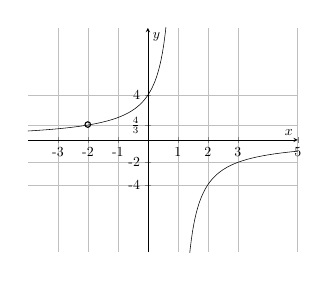
\begin{tikzpicture}[scale=0.5]
\begin{axis}[
    axis lines = middle,
    grid=major,
    legend pos={south west},
    xlabel = {$x$},
    %xlabel style={below right},
    ylabel = {$y$},
    ymin=-10,
    ymax=10,
    xmin=-4,
    xmax=5,
    xtick={-3,-2,-1,1,2,3,5},
    xticklabels={-3,-2,-1,1,2,3,5},
    ytick={-4,-2,1.333,4},
    yticklabels={-4,-2,$\frac{4}{3}$,4},
                  ]
	\addplot[domain=-4:0.99, samples=100, color=black] {4/(1-x)};
    \addplot[domain=1.01:5, samples=100, color=black] {4/(1-x)};
   % \addplot[domain=-3:3, samples=100, color=black] {-x};
     %\addlegendentry{$\text{Рис. 1}$};
\end{axis}
\draw (1.52,3.24) circle (2pt);
\end{tikzpicture}$$
б) По графику определим количество решений: $a\in\left\{0;\cfrac{4}{3}
ight\}:0,\ a\in(-\infty;0)\cup\left(0;\cfrac{4}{3}
ight)\cup\left(\cfrac{4}{3};+\infty
ight):1.$\\
